\documentclass[11pt,letter,oneside]{report}
\usepackage[pdftex]{graphicx}
\begin{document}

\title{Space Invaders}
\author{Peter Hamilton and Jared Pilcher}
\date{Fall 2011}
\maketitle

\tableofcontents

\chapter{Space Invaders Overview}
\section{History of Space Invaders}

Space invaders was a really popular game in the early 16th century.  Children played it out in the fields with the trebuchet when their parents were out of town.

Designed by Tomohiro Nishikado, Space Invaders is one of the greatest arcade games of all time.  It hold the Guinness World Record for greatest arcade game.
 

\section{Game Play}

\subsection{Objective}

The world is being invaded by marching aliens.  All of humanity has gathered behind 4 bunkers for protection.  You control the only weapons available, a supply of 3 tanks and a handful of missiles. Kill all the aliens! Watchout! The alien mothership flies over head! Destroy it at all costs!  The fate of the world rests in your hands...

Win the game by killing all of the marching aliens. Destroying the mothership gives you extra points.

\subsection{The Tank}
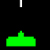
\includegraphics[]{tank.jpg}

You are the tank. Push the left button to move left, and the right button to move right. You can fire and move simultaneously.

Watchout! Enemy fire rains from above! Dodge the alien fire by moving the tank left or right. Each time your tank is hit by an alien bullet, it explodes. You have three lives.  You must survive...

Fire your missile to destroy the alien invaders! Push the middle button to fire your missile, aiming for the aliens. When the missile hits an alien, it dies. Be careful! They move left and right, and get closer as time goes on.

\subsection{Enemies}

\subsubsection{Spaceship}

\includegraphics[]{big-alien.png}

The alien mothership circles the Earth, looking for its prey. Destroy it at all costs! It flies occasionally from left to right. As it flies overhead, launch your tank missile by pushing the middle button. Be careful, it tries to evade you missile, so shoot accurately and quick!


\subsubsection{Aliens}

\includegraphics[]{aliens.jpg}

55 aliens are marching toward your position! You are charged with destroying all of them before they reach you! Fire your missiles to kill them! These aliens can shoot up to four bullets at a time. 

Aliens are capable of destroying walls, so your bunkers will provide no protection when they reach them.Their bullets slowly degrade your bunkers when their hit. Be quick! You will soon have no protection!

\subsection{Points}
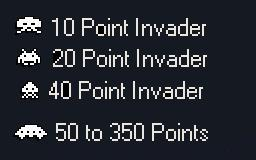
\includegraphics[]{scoring.jpg}

Earn points by destroying the aliens with your tank missiles. The lower two rows of aliens, middle two rows of aliens, and the top row of aliens are worth 10, 20 points and 40 points per alien, respectively.

Earn extra points for destroying the mothership! Earn between 50 to 350 points for each mothership destroyed.

\section{Game Details and Specifications}

\subsection{Aliens}

\subsubsection{Alien Placement and Appearance}
There are 55 enemies that start on the screen.  They are on a 11 by 5 grid.  Each grid is 15 pixels by 15 pixels.  There are three types of aliens.  The first two rows are the widest aliens, the next two rows are a little narrower and the top row has the narrowest alien.

\subsubsection{Alien Movement}
The aliens move laterally in increments of 2 pixels.  When the rightmost aliens reach the right edge of the screen, the grid of aliens will move down 7 pixels and start moving left.  When the leftmost aliens reach the left edge of the screen, they will move down 7 pixels and start moving right.  The rightmost alien and leftmost alien is the closest alien to the respective sides that has not been killed. When the rightmost column of aliens are destroyed, the aliens march toward the side of the screen until the next column hits that side. The aliens continue this pattern of movement untill the bottommost row reaches the bottom of the bunkers. The aliens will speed up in their movement as aliens are killed.

\subsubsection{Alien Explosions}
When an alien is hit by a bullet from the tank, it should blow up.  The other aliens should contiue onward while the explosion sequence is happening.

\subsection{Alien Mothership}
The alien mothership flies across the screen from left to right. It's tiem of appearance is random. When a bullet strikes the mothership, it flashes, revealing the score received.

\subsection{The Tank}
\subsubsection{Movement}
The tank moves laterally across the bottom of the screen. The user is able to push the right button to move right, or push the left button to move left at a rate of two pixels. The user is able to hold down the left or right buttons to keep the tank moving accross the screen.
\subsubsection{Firing Bullets}
You may also fire a missile by pushing the middle button. The tank is capable of moving and firing simultaneously. It is also capable of changing direction while shooting. This means that it you are able to hold down the fire button and change directins.
\subsubsection{Death}
When the tank is struct by an alien bullet, it should explode.  The player will lose a life and continue the current level.

\subsection{Bullets}
\subsubsection{Tank Bullets}
Tanks are capable of firing bullets by pushing the middle button. Tank bullets, unlike Alien Bullets, only have one appearance. They are white rectangles that are ejected just above the center of the tank. No black boxes surround the bullet. In other words, when it leaves the tank, or strikes an object, an overlay of a black box cannot be seen. When a bullet is on the screen, the tank cannot fire again until the bullet has left the screen. Each bullet travels at a distance of 2 pixels at a time. When it strikes an alien or mothership, the object is destroyed.

\subsubsection{Alien Bullets}
There are two types of alien bullets:
\begin{enumerate}
\item  Zig zag bullets rotate cyclicly through the following appearances:

\begin{enumerate}
\item 

\item 

\item >
\item 2
\end{enumerate}

\item  Cross bullets oscillate through the following appearance:

\begin{enumerate}
\item T
\item +
\item L
\end{enumerate}

\end{enumerate}

Each bullet is ejected from the center of an alien, randomly chosen to be an alien on the bottommost row. There can only be 4 bullets on the screen at any given point in time.  Once a bullet leaves the screen, a new bullet can be fired. Each bullet travels at a distance of 2 pixels at a time. When the bullet strikes a tank, it is destroyed. When the bullet strikes a bunker, the bunker is eroded. When a piece of the bunker is completely eroded, the bullet can pass through it.  No black boxes surround the bullet. In other words, when it leaves an alien, or strikes an object, an overlay of a black box cannot be seen. 
\subsection{The Bunkers}
There are four bunkers available for the tank to use as cover.  Each bunker is divided up into 10 sections.  Each section will partially erode with each collision with an alien bullet.  After 4 collisions, the section is fully eroded and will allow bullets to pass through.

When the aliens reach the bunkers, they will walk above the bunkers as they move through them.


\subsection{Scoring}
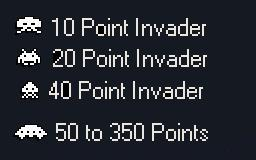
\includegraphics[]{scoring.jpg}

Earn points by destroying the aliens with your tank missiles. The lower two rows of aliens, middle two rows of aliens, and the top row of aliens are worth 10, 20 points and 40 points per alien, respectively.

\subsection{End of Game}
The game ends when one of the following three events occur:
\begin{enumerate}
\item The bottommost row of aliens that are alive reach the bottom of the bunkers.
\item The tank has been destroyed three times.
\item All aliens are destroyed.
\end{enumerate}
When the game ends, a gameover screen is displayed.

\subsection{Appearance}
The game appearance is identical to the flash version of Space Invasion. The game runs smoothly and at a decent speed. The screen is also updated close to the same rate as the flash-based game. No artifacts appear on the screen. No flickering occurs on the screen.

\chapter{Bug Reports and File Organization}

\section{Bug Reports}

\subsection{Drawing Bullets}


\subsection{One Alien Firing Two Bullets Simultaneoously}
While trying test our implementation of aliens firing bullets, we encountered a situation in which an alien fires two bullets on top of eachother.  They will appear as one bullet.  We solved this by limiting the firing of a bullet until the first one has moved out of its original position. 
\end{document}
